\documentclass[conference]{IEEEtran}
\usepackage{times}

% numbers option provides compact numerical references in the text. 
\usepackage[numbers]{natbib}
\usepackage{multicol}
\usepackage[bookmarks=true]{hyperref}
\usepackage{float}
\usepackage{graphicx}
\graphicspath{ {images/} }

\pdfinfo{
   /Author (Ron Domingo)
   /Title  (Autonomous Driving through Imitation Learning)
   /CreationDate (D:20101201120000)
   /Subject (Autonomous Driving)
   /Keywords (Autonomous Driving;CNN;Imitation Learning)
}

\begin{document}

% paper title
\title{Autonomous Driving through Imitation Learning}

% You will get a Paper-ID when submitting a pdf file to the conference system
\author{\authorblockN{Ron Domingo}
\authorblockA{Department of Electrical Engineering\\
Stanford University\\
rdomingo@stanford.edu}}


\maketitle

\begin{abstract}
The goal of this paper is to train a policy for autonomous driving via imitation learning 
that is robust enough to keep the vehicle within the drivable area while avoiding obstacles 
that may be on the road surface. Using the Duckietown driving simulator, a vehicle is trained 
by an expert to drive around a collection of training tracks with both static and dynamic obstacles.
The model is then exposed to a variety of unseen test tracks to evaluate their ability to 
drive a complete lap of each track without colliding into any obstacles or veering away from the
roads. While a highly proficient driving model was not generated due to limited expert training data,
the potential for improvement remains with future iterations of the model.
\end{abstract}

\IEEEpeerreviewmaketitle

\section{Introduction}
Path planning is a complex yet essential aspect of autonomous driving that is required
for vehicles to traverse the world around us. Finding paths is a complicated task that 
involves the avoidance of both static and dynamic obstacles, all while ensuring that the
vehicle stays within the drivable area of the road. \par
Imitation learning has become a popular method through which autonomous vehicles (AVs) are 
taught to handle the world around them. Given the complexity of the self-driving task,
traditional reinforcement learning for the self-driving problem has proven to become intractable
for the exponentially large state space associated with autonomous driving. Thus imitation learning
can significantly speed up the learning process for AVs by embedding some proper behavior within 
the learning process of the vehicle \cite{imitationLearning}. \par
This paper aims to apply imitation learning algorithms to teach an AV to drive around a closed loop
track while avoiding obstacles. The AV will be simulated using the Duckietown \cite{gym_duckietown} 
self-driving car simulator environments for OpenAI Gym. The goal of this paper is not only to
drive the simulated vehicle around Duckietown without colliding into obstacles but also to ensure
that the vehicle stays within the confines of the road surface, even when avoiding obstacles. 
The AVs will be evaluated on their ability to complete laps around various test tracks, where a 
full lap of the track without collision and off-road driving is considered a success. \par
For the purposes of the project, general road rules will not be considered when driving
around the map and purely a drivable path around the road will be considered. 

\section{Related Works}
Applying imitation learning for autonomous driving is not a novel concept, in fact, this technique
has been popularized by the research community as a way to more efficiently solve the 
autonomous driving problem, especially in comparison with reinforcement learning. \par
The paper by \citet{humanDriving} shows imitation learning being applied to path planning in an 
attempt to achieve human-like path planning from observation data. This concept is further expanded
upon in the paper by \citet{deepImitation} that created a model to perform 3D navigation through imitation
learning. Both papers apply the concepts of the imitation learning algorithm to the specific path planning 
aspect of the autonomous driving problem, however, do not yet deal with the controls of the actual 
vehicle itself. \par
Several papers have gone even further and applied models learned through imitation learning into the real 
world. The papers by \citet{agile} and \citet{waymo} have shown that imitation learning has 
merit in creating an autonomous agent that can perform in the real world. \citet{agile} demonstates
an autonomous vehicle that can drive around a high speed off-road track with a properly trained 
controller and \citet{waymo} applies imitation learning to achieve well performing driving in 
real-world scenarios. \par 
While this paper will not explicity utilize the frameworks used in each of these papers, the 
literature provides ample examples on how imitation learning can be applied to teach autonomous vehicles
how to properly drive in a more time efficient and less data intensive way. The concepts in
these papers will help to inform how the model will be formed to create a self driving agent in the 
Duckietown simulator.

\section{Setup}

\subsection{Simulation Environment}
The Duckietown self-driving car simulator is an OpenAI Gym extension that serves as a 
simulator for the Duckietown hardware robots. The driving environment features marked roads, 
intersections, static objects such as buildings and trees, and finally dynamic obstacles 
like pedestrians that move around throughout the maps randomly. \par
\begin{figure}[H]
  \centering
    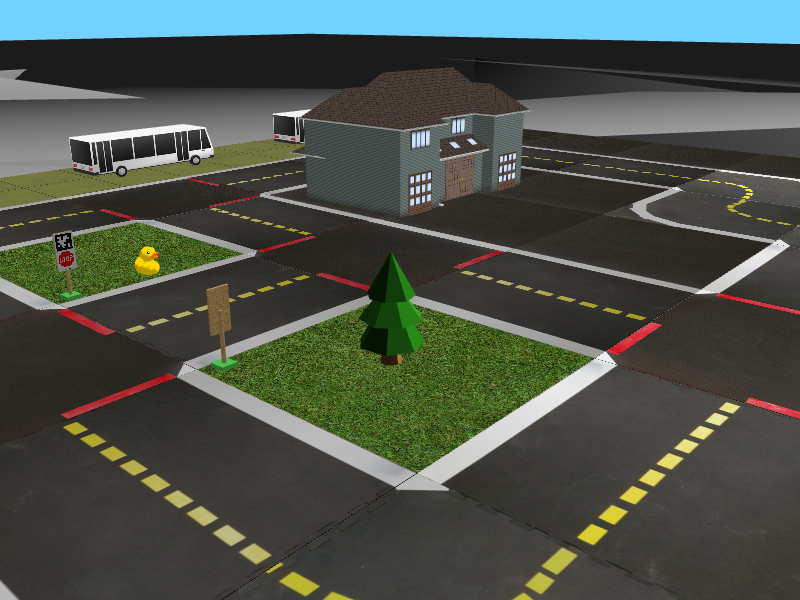
\includegraphics[scale=0.25]{simplesim_free.png}
  \caption{Simulation environment screenshot.}
\end{figure}
The Duckietown simulator outputs observations from a monocular camera mounted on the robot
with image sizes of 640x480x3 as seen in Figure \ref{fig:obs}. \par 
\begin{figure}[H]
  \centering
    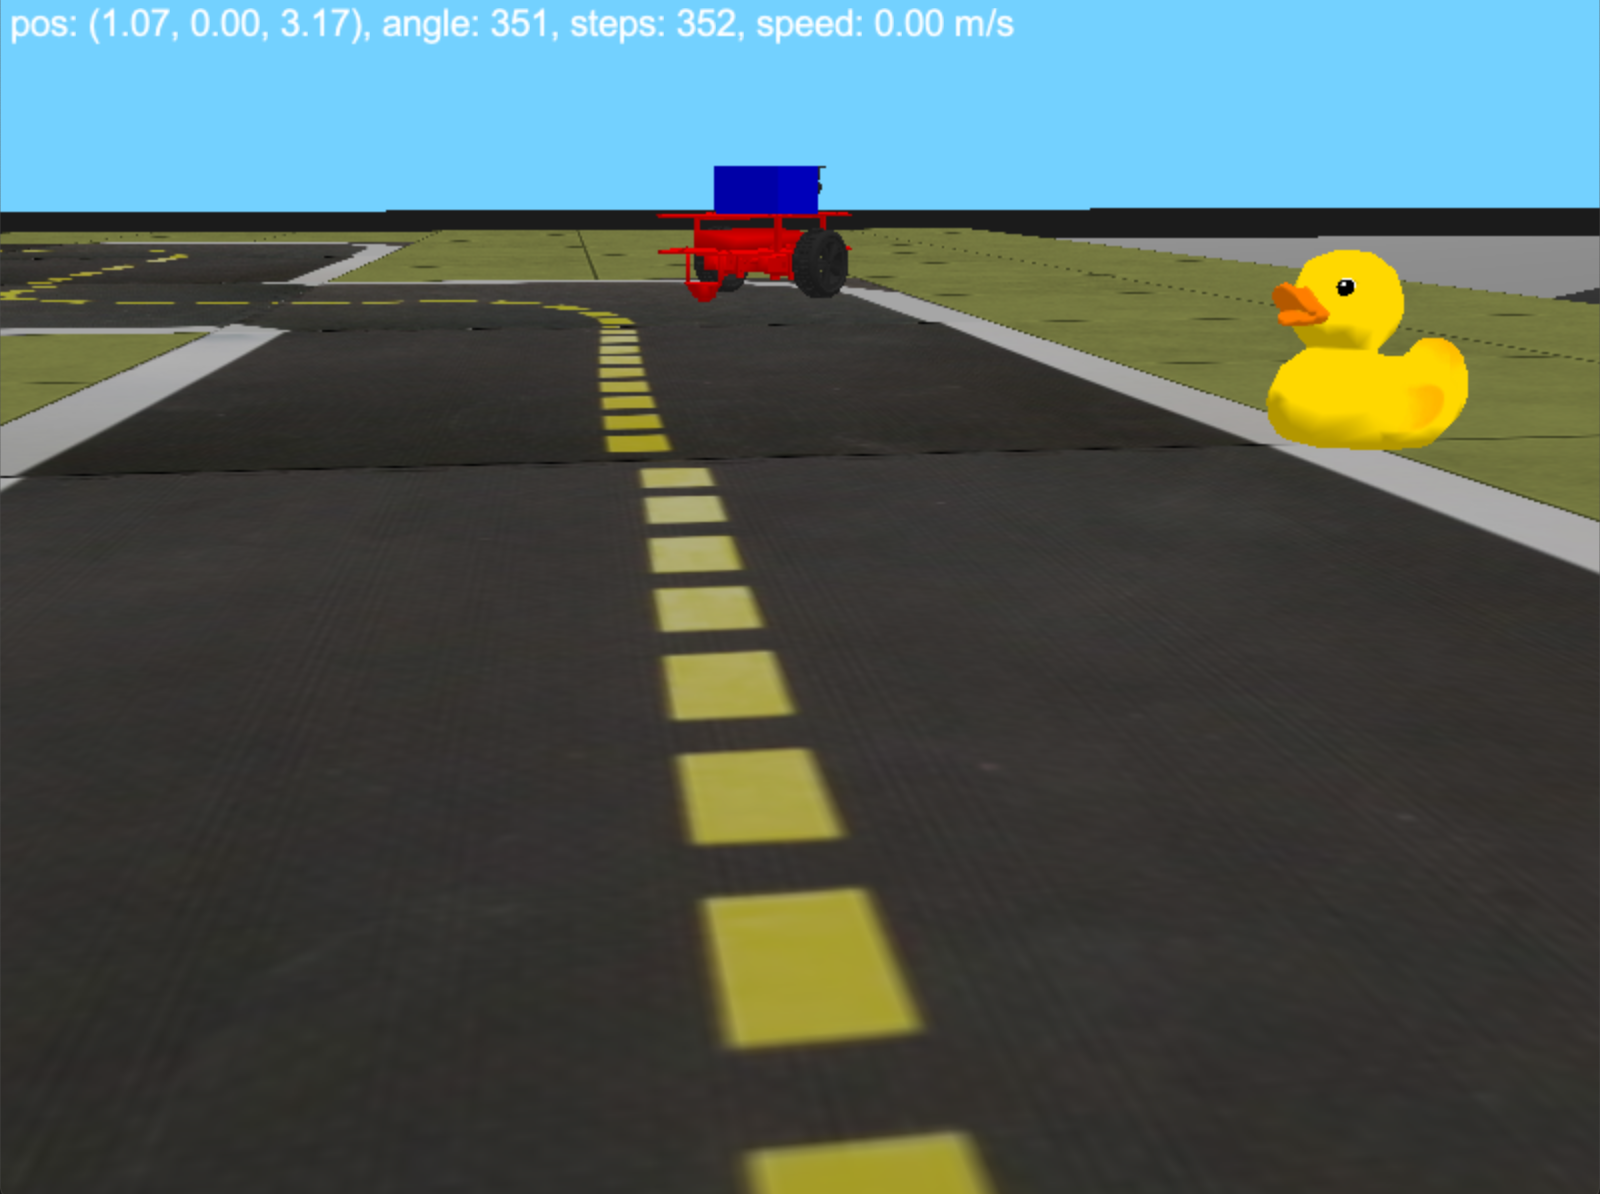
\includegraphics[scale=0.25]{first_person.png}
  \caption{Vehicle observation example.}
  \label{fig:obs}
\end{figure}
Duckietown features customizable tracks ranging from mini-cities complete with intersections, signage,
pedestrians, and buildings, to simplified straight line tracks. For the purposes of this paper,
custom closed loop tracks are considered since the AV will be evaluated on its ability to maneuver 
around the track and get back to its original positition without colliding with any obstacles along 
the way. The tracks, however, will be customized so as to provide the AV with various training and 
test tracks for evaluation. Each track will also include a collection of randomly placed obstacles 
throughout, whether they are static or dynamic obstacles on or off the road surface. This is done 
to ensure that the AV can handle maneuvers such as stopping for pedestrians or swerving around static 
objects that lie in the road. Another purpose of this randomization is to prevent the AV from simply
memorizing the tracks and different maneuvers from the testing tracks. 

\subsection{Input Processing}
The Duckietown simulator provides observations in terms of images of size 640x480x3. The first step
of image preprocessing is to downscale the images in order to improve computational efficiency. 
The observations are downscaled to a fourth of their original size through nearest-neighbor
resampling, generating images that are 160x120x3. The downscaled images are then normalized 
before being passed to the Convolutional Neural Network (CNN).

\subsection{Action Generation}
The simulation vehicle takes in two parameters for each action, the velocity and the steering angle,
each of which take on values between -1 and 1. A CNN is used to convert the raw images to the 
desired action that would enable the vehicle to get around the track.
The CNN architecture is as follows: 
\begin{itemize}
  \item Convolutional Block 
  \item Convolutional Block 
  \item Convolutional Block 
  \item Convolutional Block 
  \item Dropout
  \item Fully Connected Layer
  \item Fully Connected Layer
\end{itemize}
\begin{figure}[H]
  \centering
    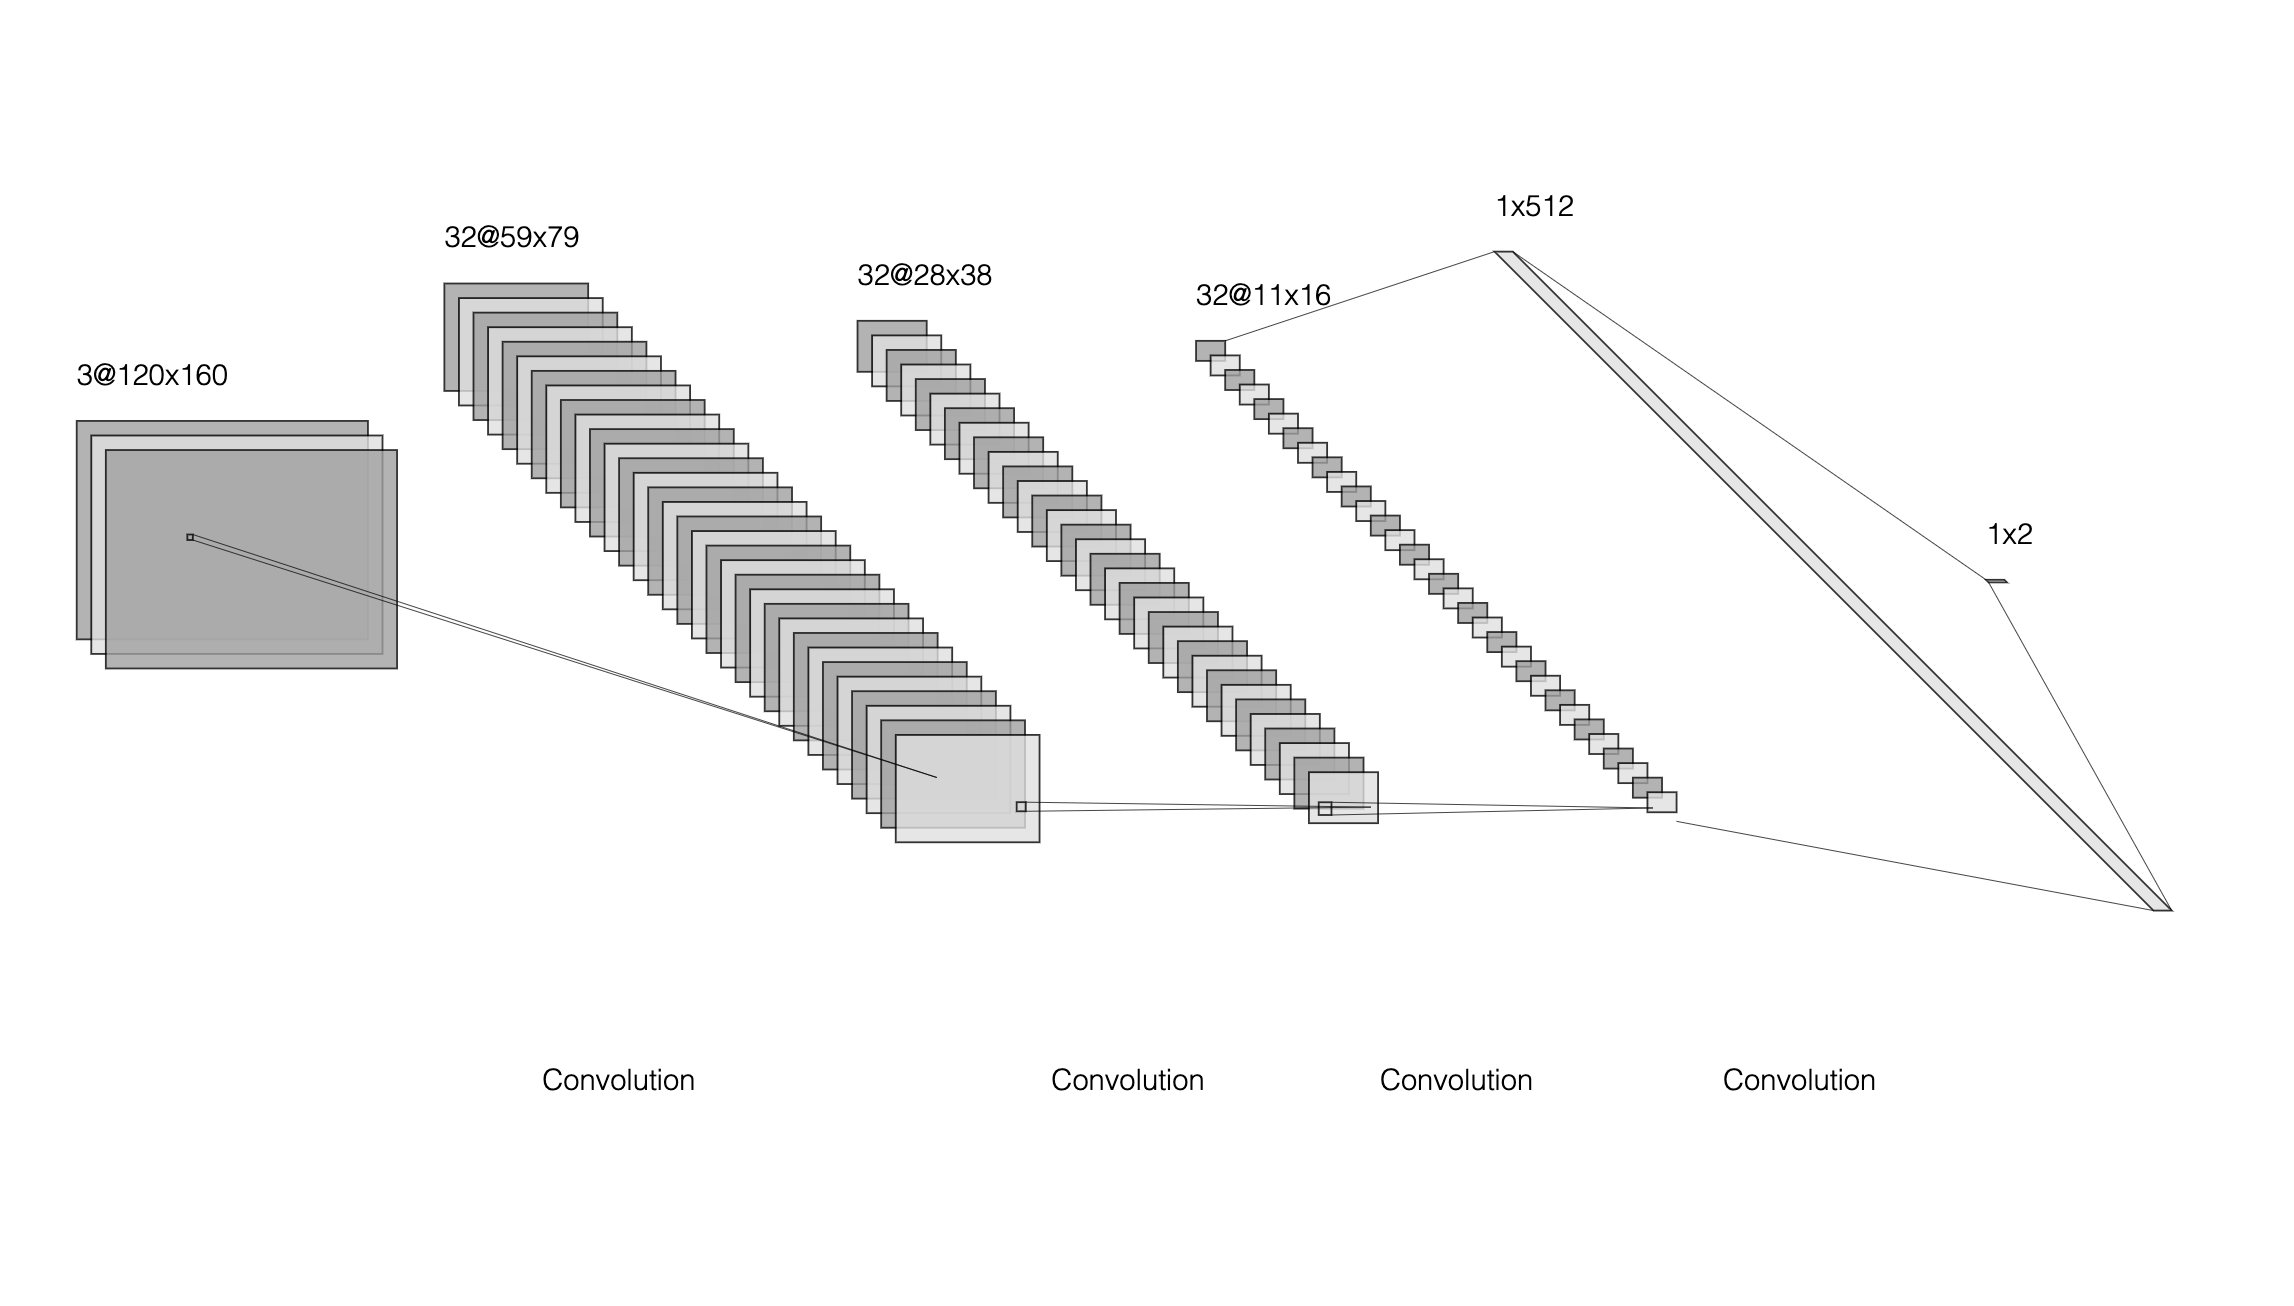
\includegraphics[scale=0.20]{neural_net.png}
  \caption{Neural Network Diagram}
\end{figure} \par
In this architecture, each convolutional block consists of a convolution, rectified linear unit, and
a batch normilization. The 4 convolutional blocks extract features from the AV camera while reducing
the state space of the image. Then information is then passed to the 2 fully connected layers to convert 
the states to the action space. \par
While the actions accepted by the simulator are continuous, the network is trained with only 
4 actions - left, right, forward, and stop. This is done to reduce the action space of the model 
and thereby reduce the computation required to perform the task at hand. \par
Two CNN models are tested throughout this paper. While both models share the same basic architecture as the
one outlined above, the models differ in their input layer. The first model uses a single camera frame
to generate an output for the vehicle, essentially utilizing an input of size 160x120x3. For the purposes 
of this paper, this model will be refered to as the single-frame model. The second
model, on the other hand, uses the current and the previous 3 frames to generate an action. These
4 frames are stacked together in order, resulting in an input size of 160x120x12. The larger input 
is an attempt to preserve some temporal relationship between the frames. The goal of the second model is 
to try and improve the driving performance given some temporal context for where the car is heading on the
track over time. In the further sections of the paper, the second model will be refered to as the multi-frame
model.


\section{Imitation Learning}
The learning process used in this paper follows the process outlined in the deep active imitation
learning paradigm by \citet{dagger}. The process is as follows: (1) Collecting demonstrations. 
(2) Supervised training of the neural network. (3) Active learning to refine the initially learned policy.
\subsection{Collecting Demonstrations}
Imitation learning requires expert behavior examples in order to train the model. For this paper, 
the expert examples were obtained from manually driving multiple laps of each test track. During 
the laps, the obvservation state and the action taken were recorded. \par
Each lap has a randomized start position and orientation and a lap is complete when the vehicle has 
reached close to its starting position on the road. Only valid laps were recorded and stored for 
training purposes. 
\subsection{Supervised Training}
Once recorded, the network is then trained on batched samples of the recorded observations and actions.
The loss function used during the training process is an L2 loss function. With the single-frame model,
batches of observations and the corresponding actions were simply taken for each training epoch. 
With the multi-frame model, preprocessing had to be done to the raw observation data. The preprocessing 
involved pre-stacking frames together in a sliding window fashion to generate a list of inputs, where each 
input were 4 frames stacked together, and their corresponding action was the action taken at the most
current frame in the stack. Both models were trained with the same expert data and each model was trained
for 100,000 epochs.
\subsection{DAGGER Re-Training}
After the supervised training has completed, each model is then run through training tracks again, but this
time autonomously. While autonomously driving, the expert user will be logging the actions they would 
have taken for any given observation. These expert actions, as well as the observations for any given 
timestep, are logged without affecting the running model so that the expert actions are attached to the 
trajectories introduced by the model when it veers off course. \par 
The models are then retrained with the new trajectories and actions to better improve the driving 
ability of the models in previously unseen trajectories.

\section{Results}
\subsection{Supervised Training}
After training both models, the training loss graphs indicate some convergence over the 
training datasets. On first inspection, the multi-frame model, in Figure \ref{fig:multi_loss},
converges much faster and with a smaller error compared to the single-frame model in Figure \ref{fig:single_loss}.
\begin{figure}[H]
  \centering
    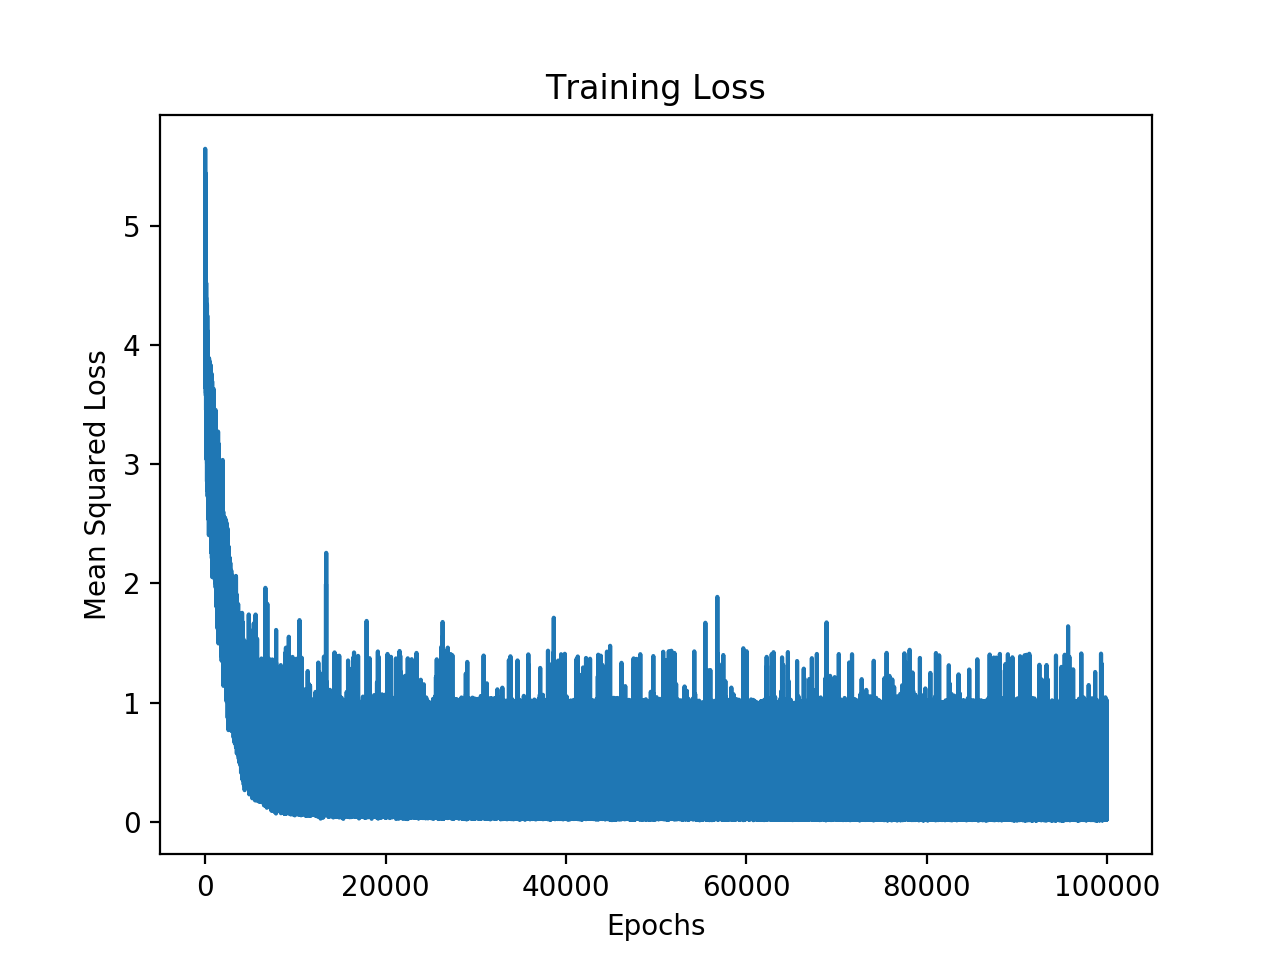
\includegraphics[scale=0.28]{single_loss.png}
  \caption{Single-frame model training loss}
  \label{fig:single_loss}
\end{figure}
\begin{figure}[H]
  \centering
    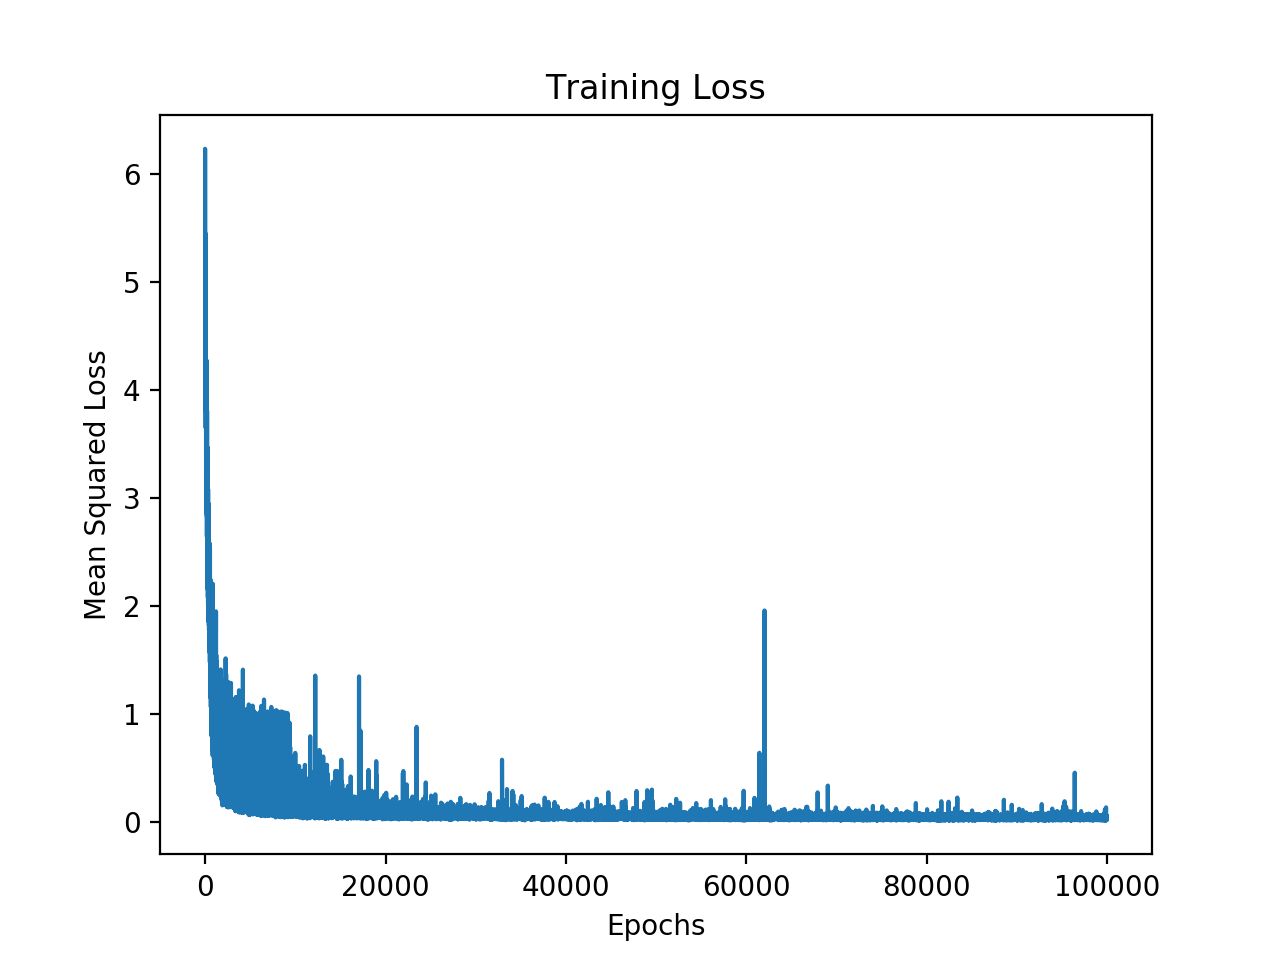
\includegraphics[scale=0.28]{window_loss.png}
  \caption{Multi-frame model training loss}
  \label{fig:multi_loss}
\end{figure}

\subsection{DAGGER Re-training}
DAGGER re-training was performed over 50,000 epochs for either model. In the case of the single-frame 
model, in Figure \ref{fig:dagger_single}, the model seemed to converge over the new DAGGER dataset, albeit with greater error than 
the training dataset. 
\begin{figure}[H]
  \centering
    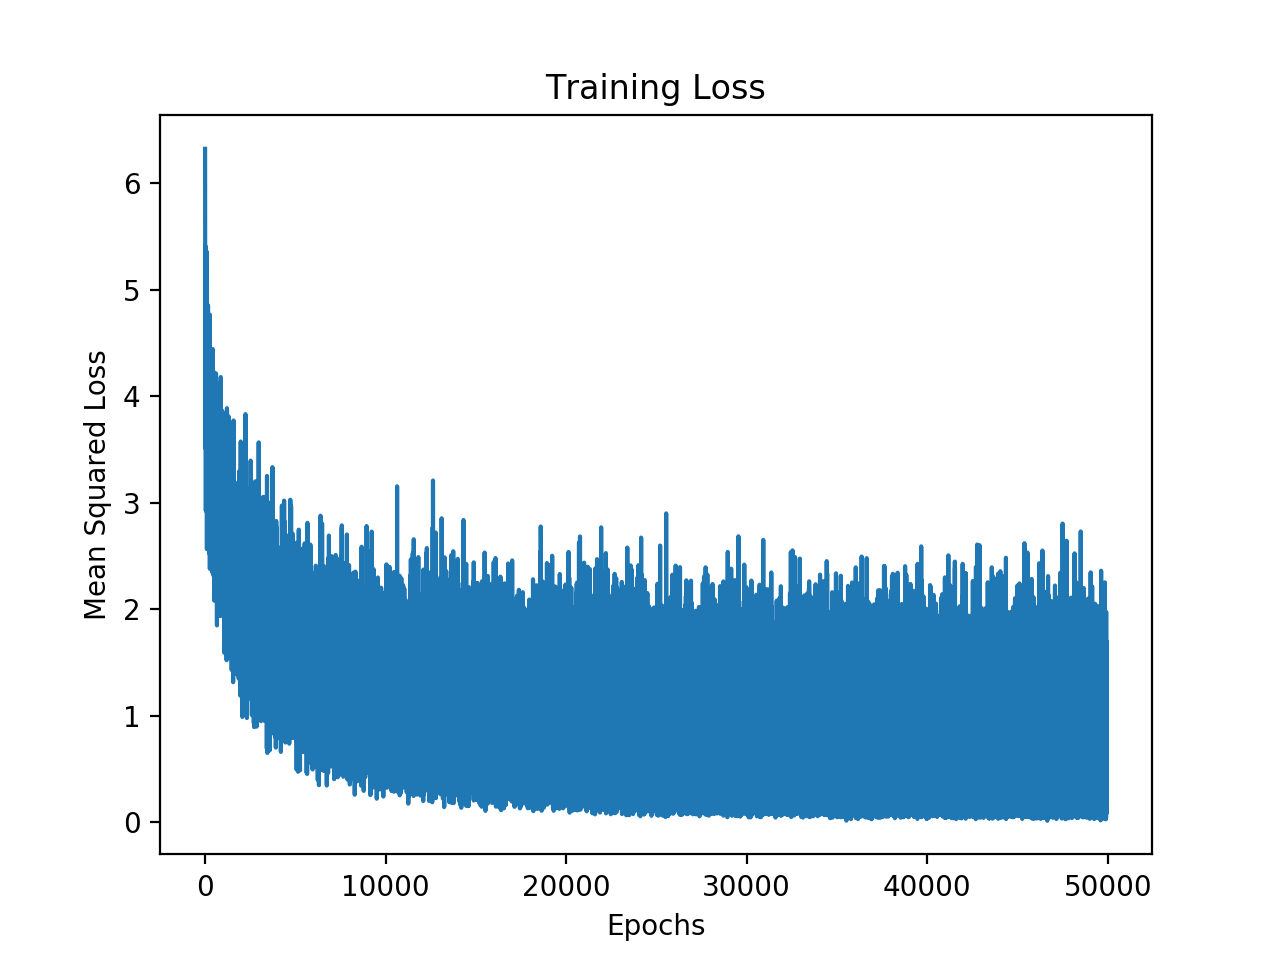
\includegraphics[scale=0.28]{single_dagger.png}
  \caption{Single-frame model DAGGER re-training loss}
  \label{fig:dagger_single}
\end{figure}
This was not the case, however, for the multi-frame model in Figure \ref{fig:dagger_multi}. After DAGGER re-training, the model does not appear
to converge over the new data and generates much larger errors than seen before, despite its low errors
in the initial supervised training.
\begin{figure}[H]
  \centering
    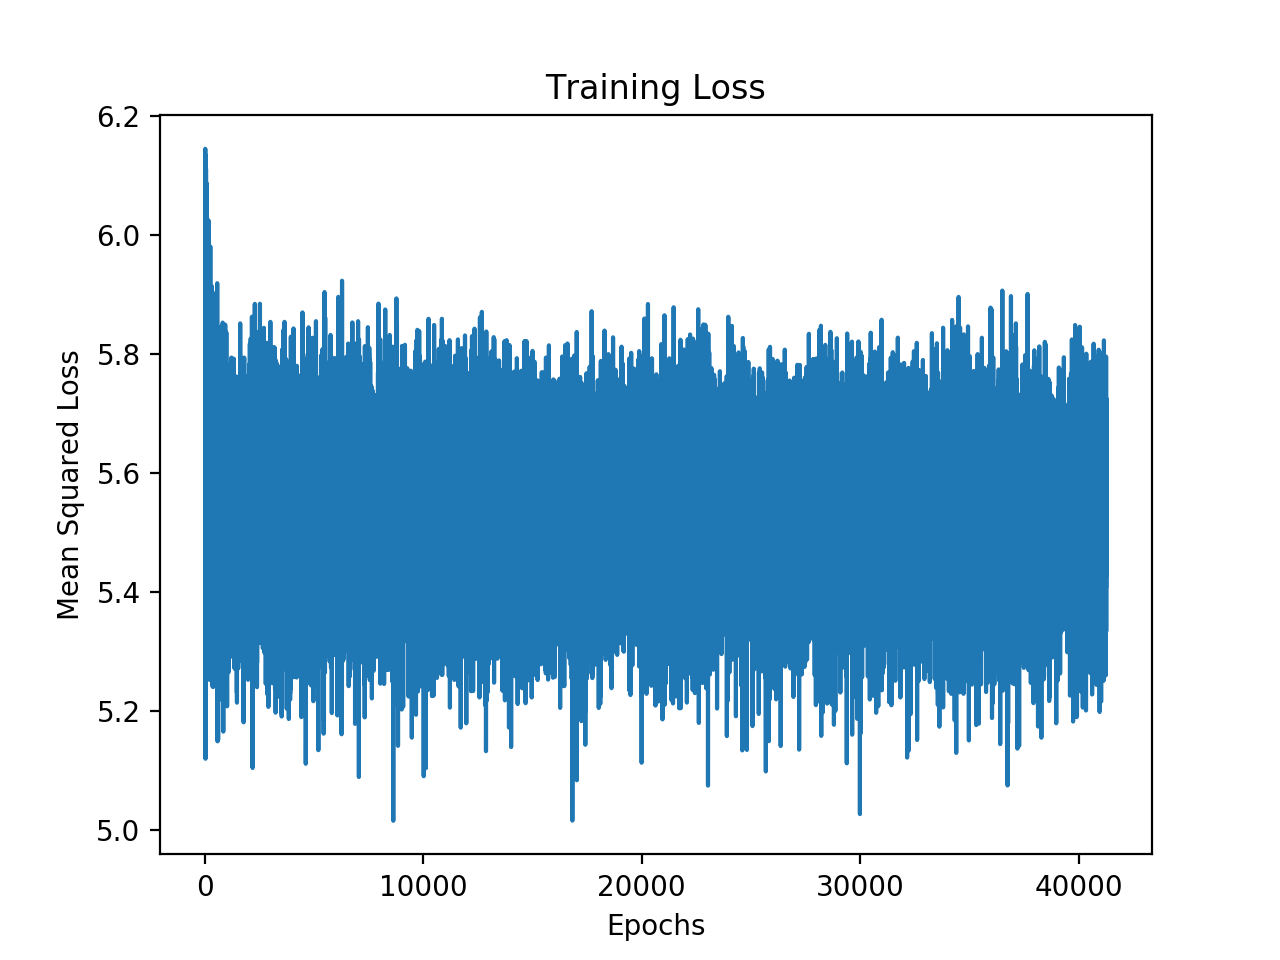
\includegraphics[scale=0.28]{multi_dagger.png}
  \caption{Multi-frame model DAGGER re-training loss}
  \label{fig:dagger_multi}
\end{figure}

\subsection{Testing}
After the training process, the models were evaluated on their ability to complete laps of unknown 
test tracks without any collisions, all while staying on the drivable area of the road. The models
were run autonomously on a variety of test tracks, each with their own distinct set of static and 
dynamic obstacles. For every failed or completed lap, the AV would respawn in a new random location 
with a random orientation. The success rate of the AVs is then recorded and used to evaluate 
the driving ability of the models. 
\subsubsection{Single-Frame Model}
The single-frame model was able to achieve a 4.5\% success rate when run over thousands of iterations
on unkown tracks. After the DAGGER re-training, the performance of the model actually decreased and 
dropped to a 0\% success rate.
\subsubsection{Multi-Frame Model}
The multi-frame model was not able to complete any successful laps when run on unknown tracks. Similarly,
after the DAGGER re-training, the multi-frame model did not improve with the corrected data.

\section{Discussion}
Overall, the two models did not perform well with unkown tracks. Most surprising is that the 
multi-frame model performed far worse than the single-frame model, despite a more promising
training loss curve. \par
The difference between the two models can be seen when watching each model drive autonomously. 
The single-frame model is able to make decisions, some correct and some not, despite having never 
seen those particular observations. This model appeared to be able to turn and keep itself on the
track rather well, but would fail in avoiding both static and dynamic obstacles on the road. \par
The multi-frame model, on the other hand, was prone to getting
stuck when faced with unseen trajectories. In these situations, the multi-frame model would either 
stop completely or drive around in circles, trying to find a road to drive on. \par
The DAGGER re-training also did not help with these behaviors. The expert action collection 
during the DAGGER algorithm has to be improved so as to provide a more accurate correction to the 
learned policies. The data for the re-training was collected with a user on a keyboard watching 
the AV drive autonomously. Without actual control of the vehicle, the user was left to hitting keys 
that they felt like would correct the vehicle trajectory, but without actual feedback, the actions
logged by the user could be mistimed and therefore incorrect. The lack of convergence in the training 
loss given the new data indicates that the new actions varied significantly from the actual expert driving
when the expert has full control of the vehicle. This is also shown by the consistent failures of the 
AVs when run on the post-DAGGER models. \par
For both models, a larger expert dataset to train on would prove extremely beneficial. The manual
collection of data proved to be a limiting factor in the performance of the trained models as a more 
comprehensive dataset with more examples of obstacle avoidance could have helped with the single-frame
model specifically. While the performance on unknown tracks was low with the single-frame model,
its performance when evaluated on the same tracks it was trained on was much better at a 37\% success rate.
This, however, could be due to memorizing the routes on those particular tracks over the unkown tracks,
although it does show some promise. The same performance can not be said for the multi-frame model
on the training tracks as it still failed to complete any successful laps on previously seen tracks.
\par 
Perhaps the poor performance of the multi-frame model was due to the fact that the attempt to incorporate
temporal information into the decision making was too naive. Instead, a full restructuring may be needed
to properly incorporate the temporal aspects of motion planning into the AV. 
This could be done by implement an LSTM network to better take advantage of temporal relationships 
between objects and the vehicle while driving around the track, as done by \citet{lstm}. 


\section{Conclusion}
\label{sec:conclusion}
Path planning is an extremely challenging issue that must be solved before vehicles can become
truly autonomous. There have been many attempts to try and solve this challenge through traditional
or deep reinforcement learning techniques, but the complexity of the problem leads to time-consuming 
and tedious methods that become cumbersome to compute. Imitation learning has gained traction over the years
as an alternative to reinforcement learning by allowing researchers to transfer human knowledge
to an agent, thereby expediting the process of obtaining well performing policies without having 
to explicitly define an extremely complex model to approximate autonomous driving. \par 
This paper applied the immitation learning algorithms to the Duckietown driving simulator 
to create an autonomous driving agent that could navigate a variety of tracks without 
any collisions all while staying within the road boundaries. Two models were tested: a model
that accepted a single camera frame and outputted an action, and a model that took in the last 
4 frames of driving to generate the best action for the vehicle. After training, the single-frame 
model fared much better than the multi-frame model, however, both models share room for 
siginificant improvement in future iterations of this project. The limited expert data greatly 
affected the driving performance of the models and the naive attempt to include temporal relationships 
in the action generation did not do much to improve performance. More work is required to 
create models that can accurately drive around the simulator with competence, but the current 
results are still significant given that the models were trained without an explicit definition 
of the problem, its rewards, the state transitions, or any ground truth actions. In this way, this 
paper was still able to show the benefits of imitation learning in trying to solve high-dimensional 
decision-making problems.

%% Use plainnat to work nicely with natbib. 

\bibliographystyle{plainnat}
\bibliography{references}

\end{document}


